\documentclass[border=1pt]{standalone}
\usepackage[T1]{fontenc}
\usepackage{mathptmx}
\usepackage{pgfplots}
\pgfplotsset{compat=1.18}
\usepgfplotslibrary{groupplots}
\definecolor{cA}{RGB}{31,119,180}\definecolor{cB}{RGB}{230,120,30}\definecolor{cC}{RGB}{44,160,44}
\definecolor{c1}{RGB}{31,119,180}\definecolor{c2}{RGB}{255,127,14}\definecolor{c3}{RGB}{44,160,44}
\definecolor{c4}{RGB}{214,39,40}\definecolor{c5}{RGB}{148,103,189}
\begin{document}

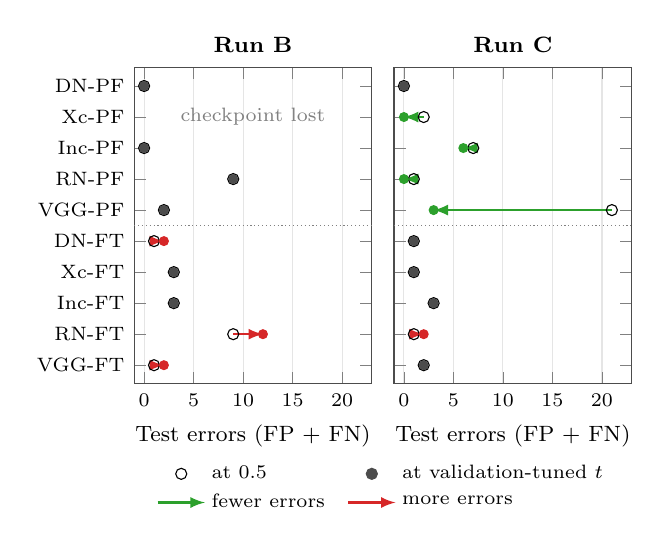
\begin{tikzpicture}
\begin{groupplot}[group style={group size=2 by 1, horizontal sep=8pt, yticklabels at=edge left},
  width=4.6cm, height=5.6cm, ymin=-0.6, ymax=9.6, ytick={0,1,2,3,4,5,6,7,8,9}, yticklabels={{VGG-FT},{RN-FT},{Inc-FT},{Xc-FT},{DN-FT},{VGG-PF},{RN-PF},{Inc-PF},{Xc-PF},{DN-PF}},
  xmin=-1, xmax=23, xtick={0,5,10,15,20}, ticklabel style={font=\scriptsize}, label style={font=\footnotesize},
  title style={font=\footnotesize\bfseries, yshift=-4pt}, xmajorgrids, grid style={black!10},
  axis line style={black!70}, xlabel={Test errors (FP + FN)},
  legend cell align=left, legend style={font=\scriptsize, draw=none, legend columns=2, at={(1.045,-0.22)}, anchor=north, /tikz/every even column/.append style={column sep=6pt}}]

\nextgroupplot[title={Run B}]
\draw[densely dotted, black!50] (axis cs:\pgfkeysvalueof{/pgfplots/xmin},4.5) -- (axis cs:\pgfkeysvalueof{/pgfplots/xmax},4.5);
\draw[-latex, c4, line width=0.8pt] (axis cs:1,0) -- (axis cs:2,0);
\addplot[only marks, mark=o, mark size=2pt, black, forget plot] coordinates {(1,0)};
\addplot[only marks, mark=*, mark size=1.6pt, c4, forget plot] coordinates {(2,0)};
\draw[-latex, c4, line width=0.8pt] (axis cs:9,1) -- (axis cs:12,1);
\addplot[only marks, mark=o, mark size=2pt, black, forget plot] coordinates {(9,1)};
\addplot[only marks, mark=*, mark size=1.6pt, c4, forget plot] coordinates {(12,1)};
\addplot[only marks, mark=o, mark size=2pt, black, forget plot] coordinates {(3,2)};
\addplot[only marks, mark=*, mark size=1.6pt, black!70, forget plot] coordinates {(3,2)};
\addplot[only marks, mark=o, mark size=2pt, black, forget plot] coordinates {(3,3)};
\addplot[only marks, mark=*, mark size=1.6pt, black!70, forget plot] coordinates {(3,3)};
\draw[-latex, c4, line width=0.8pt] (axis cs:1,4) -- (axis cs:2,4);
\addplot[only marks, mark=o, mark size=2pt, black, forget plot] coordinates {(1,4)};
\addplot[only marks, mark=*, mark size=1.6pt, c4, forget plot] coordinates {(2,4)};
\addplot[only marks, mark=o, mark size=2pt, black, forget plot] coordinates {(2,5)};
\addplot[only marks, mark=*, mark size=1.6pt, black!70, forget plot] coordinates {(2,5)};
\addplot[only marks, mark=o, mark size=2pt, black, forget plot] coordinates {(9,6)};
\addplot[only marks, mark=*, mark size=1.6pt, black!70, forget plot] coordinates {(9,6)};
\addplot[only marks, mark=o, mark size=2pt, black, forget plot] coordinates {(0,7)};
\addplot[only marks, mark=*, mark size=1.6pt, black!70, forget plot] coordinates {(0,7)};
\node[font=\scriptsize, text=black!50] at (axis cs:11,8) {checkpoint lost};
\addplot[only marks, mark=o, mark size=2pt, black, forget plot] coordinates {(0,9)};
\addplot[only marks, mark=*, mark size=1.6pt, black!70, forget plot] coordinates {(0,9)};
\addlegendimage{only marks, mark=o, black}\addlegendentry{at 0.5}
\addlegendimage{only marks, mark=*, black!70}\addlegendentry{at validation-tuned $t$}
\addlegendimage{-latex, cC, line width=0.8pt}\addlegendentry{fewer errors}
\addlegendimage{-latex, c4, line width=0.8pt}\addlegendentry{more errors}
\nextgroupplot[title={Run C}]
\draw[densely dotted, black!50] (axis cs:\pgfkeysvalueof{/pgfplots/xmin},4.5) -- (axis cs:\pgfkeysvalueof{/pgfplots/xmax},4.5);
\addplot[only marks, mark=o, mark size=2pt, black, forget plot] coordinates {(2,0)};
\addplot[only marks, mark=*, mark size=1.6pt, black!70, forget plot] coordinates {(2,0)};
\draw[-latex, c4, line width=0.8pt] (axis cs:1,1) -- (axis cs:2,1);
\addplot[only marks, mark=o, mark size=2pt, black, forget plot] coordinates {(1,1)};
\addplot[only marks, mark=*, mark size=1.6pt, c4, forget plot] coordinates {(2,1)};
\addplot[only marks, mark=o, mark size=2pt, black, forget plot] coordinates {(3,2)};
\addplot[only marks, mark=*, mark size=1.6pt, black!70, forget plot] coordinates {(3,2)};
\addplot[only marks, mark=o, mark size=2pt, black, forget plot] coordinates {(1,3)};
\addplot[only marks, mark=*, mark size=1.6pt, black!70, forget plot] coordinates {(1,3)};
\addplot[only marks, mark=o, mark size=2pt, black, forget plot] coordinates {(1,4)};
\addplot[only marks, mark=*, mark size=1.6pt, black!70, forget plot] coordinates {(1,4)};
\draw[-latex, cC, line width=0.8pt] (axis cs:21,5) -- (axis cs:3,5);
\addplot[only marks, mark=o, mark size=2pt, black, forget plot] coordinates {(21,5)};
\addplot[only marks, mark=*, mark size=1.6pt, cC, forget plot] coordinates {(3,5)};
\draw[-latex, cC, line width=0.8pt] (axis cs:1,6) -- (axis cs:0,6);
\addplot[only marks, mark=o, mark size=2pt, black, forget plot] coordinates {(1,6)};
\addplot[only marks, mark=*, mark size=1.6pt, cC, forget plot] coordinates {(0,6)};
\draw[-latex, cC, line width=0.8pt] (axis cs:7,7) -- (axis cs:6,7);
\addplot[only marks, mark=o, mark size=2pt, black, forget plot] coordinates {(7,7)};
\addplot[only marks, mark=*, mark size=1.6pt, cC, forget plot] coordinates {(6,7)};
\draw[-latex, cC, line width=0.8pt] (axis cs:2,8) -- (axis cs:0,8);
\addplot[only marks, mark=o, mark size=2pt, black, forget plot] coordinates {(2,8)};
\addplot[only marks, mark=*, mark size=1.6pt, cC, forget plot] coordinates {(0,8)};
\addplot[only marks, mark=o, mark size=2pt, black, forget plot] coordinates {(0,9)};
\addplot[only marks, mark=*, mark size=1.6pt, black!70, forget plot] coordinates {(0,9)};
\end{groupplot}
\end{tikzpicture}
\end{document}
